\section*{6. Convergence of Random Variables}\label{convergence-of-random-variables}

\subsection*{6.2 Types of convergence}\label{types-of-convergence}

\textbf{\(X_{n}\) converges to \(X\) in probability}, written
\(X_{n} \xrightarrow{\text{P}} X\), if, for every \(\epsilon > 0\),:

\[ \mathbb{P}( |X_{n} - X| > \epsilon ) \rightarrow 0 \]

as \(n \rightarrow \infty\).

\textbf{\(X_{n}\) converges to \(X\) in distribution}, written
\(X_{n} \leadsto X\), if

\[ \lim _{n \rightarrow \infty} F_{n}(t) = F(t) \]

for all \(t\) for which \(F\) is continuous.

\textbf{\(X_{n}\) converges to \(X\) in quadratic mean}, written
\(X_{n} \xrightarrow{\text{qm}} X\), if,

\[ \mathbb{E}(X_{n} - X)^{2} \rightarrow 0 \]

as \(n \rightarrow \infty\).

\textbf{Theorem 6.4}. The following relationships hold:

\begin{enumerate}[label={\arabic*.}]
\item
  \(X_{n} \xrightarrow{\text{qm}} X\) implies that
  \(X_{n} \xrightarrow{P} X\).
\item
  \(X_{n} \xrightarrow{\text{P}} X\) implies that \(X_{n} \leadsto X\).
\item
  if \(X_{n} \leadsto X\) and if \(\mathbb{P}(X = c) = 1\) for some real
  number \(c\), then \(X_{n} \xrightarrow{\text{P}} X\).
\end{enumerate}

\textbf{Proof}

\begin{enumerate}[tightlist,label={\arabic*.}]
\item
  Fix \(\epsilon > 0\). Using Chebyshev's inequality,
\end{enumerate}

\[ \mathbb{P}(|X_{n} - X| > \epsilon) = \mathbb{P}(|X_{n} - X|^{2} < \epsilon^{2}) \leq \frac{\mathbb{E}|X_{n} - X|^{2}}{\epsilon^{2}} \rightarrow 0 \]

\begin{enumerate}[tightlist,label={\arabic*.}]
\item
  Fix \(\epsilon > 0\) and let \(x\) be a point of continuity of \(F\).
  Then
\end{enumerate}

\begin{align*}
F_{n}(x) & = \mathbb{P}(X_{n} \leq x) = \mathbb{P}(X_{n} \leq x, X \leq x + \epsilon) + \mathbb{P}(X_{n} \leq x, X > x + \epsilon) \\
       & \leq \mathbb{P}(X \leq x + \epsilon) + \mathbb{P}(|X_{n} - X| > \epsilon) \\
       & = F(x + \epsilon) + \mathbb{P}(|X_{n} - X| > \epsilon)
\end{align*}

Also,

\begin{align*}
F(x - \epsilon) & = \mathbb{P}(X \leq x - \epsilon) = \mathbb{P}(X \leq x - \epsilon, X_{n} \leq x) + \mathbb{P}(X \leq x + \epsilon, X_{n} > x) \\
                & \leq F_{n}(x) + \mathbb{P}(|X_{n} - X| > \epsilon)
\end{align*}

Hence,

\[ F(x - \epsilon) - \mathbb{P}(|X_{n} - X| > \epsilon) \leq F_{n}(x) \leq F_{n}(x + \epsilon) + \mathbb{P}(|X_{n} - X| > \epsilon) \]

Take the limit as \(n \rightarrow \infty\) to conclude that

\[ F(x - \epsilon) \leq \liminf_{n \rightarrow \infty} F_{n}(x) \leq \limsup_{n \rightarrow \infty} F_{n}(x) \leq F(x + \epsilon) \]

\begin{enumerate}[tightlist,label={\arabic*.},resume]
\item
  Fix \(\epsilon > 0\). Then,
\end{enumerate}

\begin{align*}
\mathbb{P}(|X_{n} - c| > \epsilon) & = \mathbb{P}(X_{n} < c - \epsilon) + \mathbb{P}(X_{n} > c + \epsilon) \\
                                 & \leq \mathbb{P}(X_{n} \leq c - \epsilon) + \mathbb{P}(X_{n} > c + \epsilon) \\
                                 & = F_{n}(c - \epsilon) + 1 - F_{n}(c + \epsilon) \\
                                 & \rightarrow F(c - \epsilon) + 1 - F(c + \epsilon) \\
                                 & = 0 + 1 - 1 = 0
\end{align*}

Now, to show that the reverse implications do not hold:

\paragraph{Convergence in probability does not imply convergence in
quadratic
mean}\label{convergence-in-probability-does-not-imply-convergence-in-quadratic-mean}

Let \(U \sim \text{Unif}(0, 1)\), and let
\(X_{n} \sim \sqrt{n} I_{(0, 1 / n)}(U)\). Then
\(\mathbb{P}(|X_{n}| > \epsilon) = \mathbb{P}(\sqrt{n} I_{(0, 1 / n)}(U) > \epsilon) = \mathbb{P}(0 \leq U < 1/n) = 1/n \rightarrow 0\).
Hence, then \(X_{n} \xrightarrow{\text{P}} 0\). But
\(\mathbb{E}(X_{n}^{2}) = n \int_{0}^{1/n} du = 1\) for all \(n\) so \(X_{n}\)
does not converge in quadratic mean.

\paragraph{Convergence in distribution does not imply convergence in
probability}\label{convergence-in-distribution-does-not-imply-convergence-in-probability}

Let \(X \sim N(0, 1)\). Let \(X_{n} = -X\) for \(n = 1, 2, 3, \dots\);
hence \(X_{n} \sim N(0, 1)\). \(X_{n}\) has the same distribution as \(X\)
for all \(n\) so, trivially, \(\lim _{n} F_{n}(x) \rightarrow F(x)\) for all
\(x\). Therefore, \(X_{n} \leadsto X\). But
\(\mathbb{P}(|X_{n} - X| > \epsilon) = \mathbb{P}(|2X| > \epsilon) \neq 0\).
So \(X_{n}\) does not tend to \(X\) in probability.

\begin{figure}[H]
\centering
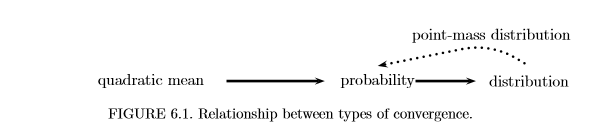
\includegraphics[keepaspectratio]{Figure-06-01}
\caption{Figure-06-01}
\end{figure}

\textbf{Theorem 6.5} Let \(X_{n}, X, Y_{n}, Y\) be random variables. Let
\(g\) be a continuous function. Then:

\begin{enumerate}[tightlist,label={\arabic*.}]
\item
  If \(X_{n} \xrightarrow{\text{P}} X\) and
  \(Y_{n} \xrightarrow{\text{P}} Y\), then
  \(X_{n} + Y_{n} \xrightarrow{\text{P}} X + Y\).
\item
  If \(X_{n} \xrightarrow{\text{qm}} X\) and
  \(Y_{n} \xrightarrow{\text{qm}} Y\), then
  \(X_{n} + Y_{n} \xrightarrow{\text{qm}} X + Y\).
\item
  If \(X_{n} \leadsto X\) and \(Y_{n} \leadsto c\), then
  \(X_{n} + Y_{n} \leadsto X + c\).
\item
  If \(X_{n} \xrightarrow{\text{P}} X\) and
  \(Y_{n} \xrightarrow{\text{P}} Y\), then
  \(X_{n} Y_{n} \xrightarrow{\text{P}} XY\).
\item
  If \(X_{n} \leadsto X\) and \(Y_{n} \leadsto c\), then
  \(X_{n} Y_{n} \leadsto cX\).
\item
  If \(X_{n} \xrightarrow{\text{P}} X\) then
  \(g(X_{n}) \xrightarrow{\text{P}} g(X)\) .
\item
  If \(X_{n} \leadsto X\) then \(g(X_{n}) \leadsto g(X)\).
\end{enumerate}

\subsection*{6.3 The Law of Large
Numbers}\label{the-law-of-large-numbers}

\textbf{Theorem 6.6 (The Weak Law of Large Numbers (WLLN))}. If
\(X_{1}, X_{2}, \dots, X_{n}\) are IID, then
\(\overline{X}_{n} \xrightarrow{\text{P}} \mu\).

\textbf{Proof}: Assume that \(\sigma < \infty\). This is not necessary
but it simplifies the proof. Using Chebyshev's inequality,

\[ \mathbb{P}(|\overline{X}_{n} - \mu| > \epsilon) \leq \frac{\mathbb{E}(|\overline{X}_{n} - \mu|^{2})}{\epsilon^{2}} = \frac{\mathbb{V}(\overline{X}_{n})}{\epsilon^{2}} = \frac{\sigma^{2}}{n \epsilon^{2}} \]

which tends to 0 as \(n \rightarrow \infty\).

\subsection*{6.4 The Central Limit
Theorem}\label{the-central-limit-theorem}

\textbf{Theorem 6.8 (The Central Limit Theorem (CLT))}. Let
\(X_{1}, X_{2}, \dots, X_{n}\) be IID with mean \(\mu\) and variance
\(\sigma^{2}\). Let \(\overline{X}_{n} = n^{-1}\sum_{i=1}^{n} X_{i}\). Then

\[ Z_{n} \equiv \frac{\sqrt{n} \left( \overline{X}_{n} - \mu \right)}{\sigma} \leadsto Z \]

where \(Z \sim N(0, 1)\). In other words,

\[ \lim _{n \rightarrow \infty} \mathbb{P}(Z_{n} \leq z) = \Phi(z) = \int _{-\infty} ^z \frac{1}{\sqrt{2 \pi}} e^{-x^{2}/2}dx\]

In addition to \(Z_{n} \leadsto N(0, 1)\), there are several forms of
notation to denote the fact that the distribution of \(Z_{n}\) is
converging to a Normal. They all mean the same thing. Here they are:

\begin{align*}
Z_{n}                                           & \approx N(0, 1) \\
\overline{X}_{n}                                & \approx N\left( \mu, \frac{\sigma^{2}}{n} \right)  \\
\overline{X}_{n} - \mu                          & \approx N\left( 0,   \frac{\sigma^{2}}{n} \right)  \\
\sqrt{n}(\overline{X}_{n} - \mu)                & \approx N\left( 0, \sigma^{2} \right)              \\
\frac{\sqrt{n}(\overline{X}_{n} - \mu)}{\sigma} & \approx N(0, 1)
\end{align*}

The central limit Theorem tells us that
\(Z_{n} = \sqrt{n}(\overline{X}_{n} - \mu)/\sigma\) is approximately
\(N(0, 1)\). However, we rarely know \(\sigma\). We can estimate
\(\sigma^{2}\) from \(X_{1}, X_{2}, \dots, X_{n}\) by

\[ S_{n}^{2} = \frac{1}{n - 1} \sum_{i=1}^{n} ( X_{i} - \overline{X}_{n} )^{2} \]

This raises the following question: if we replace \(\sigma\) with
\(S_{n}\) is the central limit Theorem still true? The answer is yes.

\textbf{Theorem 6.10}. Assume the same conditions as the CLT. Then,

\[ \frac{\sqrt{n} \left(\overline{X}_{n} - \mu \right)}{S_{n}} \leadsto N(0, 1)\]

You might wonder how accurate the normal approximation is. The answer is
given by the Berry-Essèen Theorem.

\textbf{Theorem 6.11 (Berry-Essèen)}. Suppose that
\(\mathbb{E}|X_{1}|^{3} < \infty\). Then

\[ \sup _z |\mathbb{P}(Z_{n} \leq z) - \Phi(z)| \leq \frac{33}{4} \frac{\mathbb{E}|X_{1} - \mu|^{3}}{\sqrt{n}\sigma^{3}} \]

There is also a multivariate version of the central limit Theorem.

\textbf{Theorem 6.12 (Multivariate central limit Theorem)}. Let
\(X_{1}, \dots, X_{n}\) be IID random vectors where

\[ X_{i} = \begin{pmatrix} X_{1i} \\ X_{2i} \\ \vdots \\ X_{ki} \end{pmatrix}\]

with mean

\[ \mu 
= \begin{pmatrix} \mu_{1} \\ \mu_{2} \\ \vdots \\ \mu_{k} \end{pmatrix} 
= \begin{pmatrix} \mathbb{E}(X_{1i}) \\ \mathbb{E}(X_{2i}) \\ \vdots \\ \mathbb{E}(X_{ki}) \end{pmatrix} \]

and variance matrix \(\Sigma\). Let

\[ \overline{X} = \begin{pmatrix} \overline{X}_{1} \\ \overline{X}_{2} \\ \vdots \\ \overline{X}_{k} \end{pmatrix}\]

where $\overline{X} r = n^{-1} \sum_{i=1}^{n} X_{ri}
$. Then,

\[ \sqrt{n} (\overline{X} - \mu) \leadsto N(0, \Sigma) \]

\subsection*{6.5 The Delta Method}\label{delta:method}

\textbf{Theorem 6.13 (The Delta Method)}. Suppose that

\[ \frac{\sqrt{n}(Y_{n} - \mu)}{\sigma} \leadsto N(0, 1)\]

and that \(g\) is a differentiable function such that \(g'(u) \neq 0\).
Then

\[ \frac{\sqrt{n}(g(Y_{n}) - g(u))}{|g'(u)| \sigma} \leadsto N(0, 1)\]

In other words,

\[ Y_{n} \approx N \left( \mu, \frac{\sigma^{2}}{n} \right) \Rightarrow g(Y_{n}) \approx N \left( g(\mu), (g'(\mu))^{2} \frac{\sigma^{2}}{n} \right) \]

\textbf{Theorem 6.15 (The Multivariate Delta method)}. Suppose that
\(Y_{n} = (Y_{n1}, \dots, Y_{nk})\) is a sequence of random vectors such
that

\[ \sqrt{n}(Y_{n} - \mu) \leadsto N(0, \Sigma) \]

Let \(g : \mathbb{R}^{k} \rightarrow \mathbb{R}\) and let

\[ \nabla g = \begin{pmatrix} \frac{\partial g}{\partial y_{1}} \\ \vdots \\  \frac{\partial g}{\partial y_{k}} \end{pmatrix} \]

Let \(\nabla_\mu\) denote \(\nabla g(y)\) evaluated at \(y = \mu\) and
assume that the elements of \(\nabla_\mu\) are non-zero. Then

\[ \sqrt{n}(g(Y_{n}) - g(\mu)) \leadsto N(0, \nabla_\mu^T \Sigma \nabla_\mu) \]

\subsection*{6.6 Technical appendix}

\textbf{\(X_{n}\) converges to \(X\) almost surely}, written
\(X_{n} \xrightarrow{\text{as}} X\), if

\[ \mathbb{P}(\{s : X_{n}(s) \rightarrow X(s)\}) = 1 \]

\textbf{\(X_{n}\) converges to \(X\) in \(L_{1}\)}, written
\(X_{n} \xrightarrow{L_{1}} X\), if

\[ \mathbb{E} |X_{n} - X| \rightarrow 0 \]

\textbf{Theorem 6.17}. Let \(X_{n}\) and \(X\) be random variables. Then:

\begin{enumerate}[tightlist,label={\arabic*.}]
\item
  \(X_{n} \xrightarrow{\text{as}} X\) implies that
  \(X_{n} \xrightarrow{\text{P}} X\).
\item
  \(X_{n} \xrightarrow{\text{qm}} X\) implies that
  \(X_{n} \xrightarrow{L_{1}} X\).
\item
  \(X_{n} \xrightarrow{L_{1}} X\) implies that
  \(X_{n} \xrightarrow{\text{P}} X\).
\end{enumerate}

The weak law of large numbers says that \(\overline{X}_{n}\) converges to
\(\mathbb{E} X\) in probability. The strong law asserts that this is
also true almost surely.

\textbf{Theorem 6.18 (The strong law of large numbers)}. Let
\(X_{1}, X_{2}, \dots, X_{n}\) be IID. If \(\mu = \mathbb{E}|X_{1}| < \infty\)
then \(\overline{X}_{n} \xrightarrow{\text{as}} \mu\).

A sequence is \textbf{asymptotically uniformly integrable} if

\[ \lim _{M \rightarrow \infty} \limsup _{n \rightarrow \infty} \mathbb{E} ( |X_{n}| I(|X_{n}| > M) ) = 0 \]

If \(X_{n} \xrightarrow{\text{P}} b\) and \(X_{n}\) is asymptotically
uniformly integrable, then \(\mathbb{E}(X_{n}) \rightarrow b\).

The \textbf{moment generating function} of a random variable \(X\) is

\[\psi_X(t) = \mathbb{E}(e^{tX}) = \int_u e^{tu} f_X(u) du\]

\textbf{Lemma 6.19}. Let \(Z_{1}, Z_{2}, \dots, Z_{n}\) be a sequence of
random variables. Let \(\psi_{n}\) be the mgf of \(Z_{n}\). Let \(Z\) be
another random variable and denote its mgf by \(\psi\). If
\(\psi_{n}(t) \rightarrow \psi(t)\) for all \(t\) in some open interval
around 0, then \(Z_{n} \leadsto Z\).

\paragraph{Proof of the Central Limit
Theorem}\label{proof-of-the-central-limit-Theorem}

Let \(Y_{i} = (X_{i} - \mu) / \sigma\). Then, \(Z_{n} = n^{-1/2} \sum_{i} Y_{i}\).
Let \(\psi(t)\) be the mgf of \(Y_{i}\). The mgf of \(\sum_{i} Y_{i}\) is
\((\psi(t))^{n}\) and the mgf of \(Z_{n}\) is
\([\psi(t / \sqrt{n})]^{n} \equiv \xi_{n}(t)\).

Now \(\psi'(0) = \mathbb{E}(Y_{1}) = 0\) and
\(\psi''(0) = \mathbb{E}(Y_{1}^{2}) = \mathbb{V}(Y_{1}) = 1\). So,

\begin{align*}
\psi(t) & = \psi(0) + t \psi'(0) + \frac{t^{2}}{2!} \psi''(0) + \frac{t^{3}}{3!} \psi'''(0) + \dots \\
        & = 1 + 0 + \frac{t^{2}}{2} +  \frac{t^{3}}{3!} \psi'''(0) + \ldots \\
        & = 1 + \frac{t^{2}}{2} +  \frac{t^{3}}{3!} \psi'''(0) + \ldots
\end{align*}

Now,

\begin{align*}
\xi_{n}(t) & = \left[ \psi \left( \frac{t}{\sqrt{n}} \right) \right] ^{n} \\
         & = \left[  1 + \frac{t^{2}}{2n} +  \frac{t^{3}}{3!n^{3/2}} \psi'''(0) + \ldots \right] ^{n} \\
         & = \left[  1 + \frac{\frac{t^{2}}{2} +  \frac{t^{3}}{3!n^{1/2}} \psi'''(0) + \ldots}{n} \right] ^{n} \\
         & \rightarrow e^{t^{2}/2}
\end{align*}

which is the mgf of \(N(0, 1)\). The resolt follows from the previous
Theorem. In the last step we used the fact that, if
\(a_{n} \rightarrow a\), then

\[ \left( 1 + \frac{a_{n}}{n} \right) ^{n} \rightarrow e^{a} \]

\subsection*{6.8 Exercises}

\textbf{Exercise 6.8.1.} Let \(X_{1}, \dots, X_{n}\) be iid with finite mean
\(\mu = \mathbb{E}(X_{i})\) and finite variance
\(\sigma^{2} = \mathbb{V}(X_{i})\). Let \(\overline{X}_{n}\) be the sample
mean and let \(S_{n}^{2}\) be the sample variance.

\textbf{(a)} Show that \(\mathbb{E}(S_{n}^{2}) = \sigma^{2}\).

\textbf{Solution}:

\(S_{n}^{2}\) is the sample variance, that is, $ S_{n}^{2} =
(n-1)^{-1} \sum_{i=1}^{n} ( X\_{i} - \overline{X}_{n})^{2} $.
Therefore:

\begin{align*}
\mathbb{E}[S_{n}^{2}] & = \mathbb{E}\left[ \frac {1}{n-1} \sum_{i=1}^{n} \left(X_{i} - \overline{X}_{n} \right)^{2} \right] \\
& = \frac {1}{n-1} \mathbb{E} \left( \sum_{i=1}^{n} X_{i}^{2} - 2 \overline{X}_{n} \sum_{i=1}^{n} X_{i} + \sum_{i=1}^{n} \overline{X}_{n}^{2} \right) \\
& = \frac {1}{n-1} \mathbb{E} \left( \sum_{i=1}^{n} X_{i}^{2} - 2 n \overline{X}_{n}^{2} + n \overline{X}_{n}^{2} \right) \\
& = \frac {n}{n-1} \left[ \mathbb{E} (X_{i}^{2}) - \mathbb{E} \overline{X}_{n}^{2} \right] \\
& = \frac {n}{n-1} \left[ \left( \mu^{2}+\sigma^{2} \right) - \left( \mu^{2} + \frac {\sigma^{2}}{n} \right) \right] \\
& = \sigma^{2}
\end{align*}

\textbf{(b)} Show that \(S_{n}^{2} \xrightarrow{\text{P}} \sigma^{2}\).

Hint: show that
\(S_{n}^{2} = c_{n} n^{-1} \sum_{i=1}^{n} X_{i}^{2} - d_{n} \overline{X}_{n}^{2}\) where
\(c_{n} \rightarrow 1\) and \(d_{n} \rightarrow 1\). Apply the law of large
numbers to \(n^{-1}\sum_{i=1}^{n} X_{i}^{2}\) and to \(\overline{X}_{n}\). Then
use part (e) of Theorem 6.5.

\textbf{Solution}:

Similar to derivation in \textbf{(a)} we have:

\begin{align*}
S_{n}^{2} & = \frac {1}{n-1} \left( \sum_{i=1}^{n} X_{i}^{2} - n \overline{X}_{n}^{2} \right) \\
& = \frac{n}{n-1} \frac{1}{n} \sum_{i=1}^{n} X_{i}^{2} - \frac{n}{n-1} \overline{X}_{n}^{2} 
\end{align*}

where \(c_{n} = d_{n} = \frac{n}{n-1} \rightarrow 1\).

Applying the law of large numbers to \(X_{i}^{2}\):

\[ n^{-1} \sum_{i=1}^{n} X_{i}^{2} \xrightarrow{\text{P}} \mathbb{E}(X_{i}^{2}) = \sigma^{2} + \mu^{2}\]

\[ \overline{X}_{n} \xrightarrow{\text{P}} \mathbb{E}(X_{i}) = \mu \Rightarrow \overline{X}_{n}^{2} \xrightarrow{\text{P}} \mu^{2} \]

Therefore, from Theorem 6.5.e, $ S_{n}^{2} = c_{n} n^{-1}
\sum_{i=1}^{n} X_{i}^{2} - d_{n} \overline{X}_{n}^{2}
\xrightarrow{\text{P}} \sigma^{2} + \mu^{2} - \mu^{2} =
\sigma^{2}$.

\textbf{Exercise 6.8.2.} Let \(X_{1}, X_{2}, \dots, X_{n}\) be a sequence of
random variables. Show that \(X_{n} \xrightarrow{\text{qm}} b\) if and
only if

\begin{align*}\lim_{n \rightarrow \infty} \mathbb{E}(X_{n}) = b
\quad\mathrm{and}\quad 
\lim_{n \rightarrow \infty} \mathbb{V}(X_{n}) = 0
\end{align*}

\textbf{Solution}:

\(X_{n} \xrightarrow{\text{qm}} b\) id equivalent to:

\begin{align*}
\mathbb{E}[(X_{n} - b)^{2}]           & \rightarrow 0 \\
\mathbb{E}[X_{n}^{2} - 2b X_{n} + b^{2}]  & \rightarrow 0 \\
\mathbb{E}[X_{n}^{2}] - 2b \mathbb{E}[X_{n}] + b^{2} & \rightarrow 0 \\
\mathbb{E}[X_{n}^{2}] - 2b \mathbb{E}[X_{n}] + b^{2} & \rightarrow 0 \\
\mathbb{V}[X_{n}] + (\mathbb{E}[X_{n}])^{2} - 2b \mathbb{E}[X_{n}] + b^{2}  & \rightarrow 0
\end{align*}

If \(\lim_{n \rightarrow \infty} \mathbb{V}[X_{n}] = 0\) and
\(\lim_{n \rightarrow \infty} \mathbb{E}[X_{n}] = b\), then

\begin{align*}
& \lim_{n \rightarrow \infty} \mathbb{E}[(X_{n} - b)^{2}] = \\
& = \lim_{n \rightarrow \infty} \mathbb{V}[X_{n}] + (\mathbb{E}[X_{n}])^{2} - 2b \mathbb{E}[X_{n}] + b^{2} \\
& = \lim_{n \rightarrow \infty} \mathbb{V}[X_{n}] + (\lim_{n \rightarrow \infty} \mathbb{E}[X_{n}])^{2} - 2b \lim_{n \rightarrow \infty} \mathbb{E}[X_{n}] + b^{2} \\
&= 0 + b^{2} - 2b^{2} + b^{2} \\
&= 0
\end{align*}

On the other direction, if \(X_{n} \xrightarrow{\text{qm}} b\), then

\begin{align*}
\lim_{n \rightarrow \infty} \mathbb{V}[X_{n}] + (\lim_{n \rightarrow \infty} \mathbb{E}[X_{n}])^{2} - 2b \lim_{n \rightarrow \infty} \mathbb{E}[X_{n}] + b^{2} &= 0 \\
\lim_{n \rightarrow \infty} \mathbb{V}[X_{n}] + (\lim_{n \rightarrow \infty} \mathbb{E}[X_{n}] - b)^{2} &= 0 \\
\lim_{n \rightarrow \infty} \mathbb{V}[X_{n} - b] + \lim_{n \rightarrow \infty}  (\mathbb{E}[X_{n} - b])^{2} &= 0
\end{align*}

Since both terms inside the limits are non-negative, the limits
themselves are non-negative. Two non-negative values add up to 0, so
they must both be zero, and so we have:

\begin{align*}\lim_{n \rightarrow \infty} \mathbb{E}(Y_{n}) = 0
\quad\mathrm{and}\quad 
\lim_{n \rightarrow \infty} \mathbb{V}(Y_{n}) = 0
\end{align*}

or, equivalently,

\begin{align*}\lim_{n \rightarrow \infty} \mathbb{E}(X_{n}) = b
\quad\mathrm{and}\quad 
\lim_{n \rightarrow \infty} \mathbb{V}(X_{n}) = 0
\end{align*}

\textbf{Exercise 6.8.3}. Let \(X_{1}, X_{2}, \dots, X_{n}\) be iid and let
\(\mu = \mathbb{E}(X_{i})\). Suppose that variance is finite. Show that
\(\overline{X}_{n} \xrightarrow{\text{qm}} \mu\).

\textbf{Solution}.

Let \(Y_{i} = X_{i} - \mu\). It has variance \(\sigma_Y = \sigma\) and mean
\(\mu_Y = 0\). We have:

\begin{align*}
& \mathbb{E}[(\overline{X}_{n} - \mu)^{2}] = \\
& = \mathbb{E}\left[\left(\frac{1}{n} \sum_{i=1}^{n} (X_{i} - \mu) \right)^{2}\right] \\
& = \frac{1}{n^{2}} \mathbb{E} \left[ \left(\sum_{i=1}^{n} Y_{i} \right)^{2} \right] \\
& = \frac{1}{n^{2}} \left( \sum_{i=1}^{n} \mathbb{E}[Y_{i}^{2}] - \sum_{i=1}^{n} \sum_{j=1, j \neq i}^{n} \mathbb{E}[Y_{i} Y_{j}] \right) \\
& = \frac{1}{n} \left( (\sigma_Y^{2} + \mu_Y^{2}) - (n-1) \mu_Y^{2} \right) \\
& = \frac{\sigma}{n}
\end{align*}

Therefore,
\(\lim _{n \rightarrow \infty} \mathbb{E}[(\overline{X}_{n} - \mu)^{2}] = \lim _{n \rightarrow \infty} \sigma / n = 0\),
and so \(\overline{X}_{n} \xrightarrow{\text{qm}} \mu\).

\textbf{Exercise 6.8.4}. Let \(X_{1}, X_{2}, \dots\) be a sequence of random
variables such that

\begin{align*}\mathbb{P}\left(X_{n} = \frac{1}{n}\right) = 1 - \frac{1}{n^{2}}
\quad\mathrm{and}\quad 
\mathbb{P}\left(X_{n} = n\right) = \frac{1}{n^{2}}
\end{align*}

Does \(X_{n}\) converge in probability? Doex \(X_{n}\) converge in quadratic
mean?

\textbf{Solution}.

For any distribution \(X\), we have:

\begin{align*}
& \mathbb{P}( |X_{n} - X| > \epsilon ) = \\
&= \mathbb{P}\left( |X_{n} - X| > \epsilon \;\middle|\; X_{n} = \frac{1}{n} \right)\mathbb{P}\left(X_{n} = \frac{1}{n}\right)
  + \mathbb{P}\left( |X_{n} - X| > \epsilon \;\middle|\; X_{n} = n \right)\mathbb{P}\left(X_{n} = n\right) \\
&= \mathbb{P}\left( \middle|\frac{1}{n} - X\middle|\; > \epsilon \right)\left(1 - \frac{1}{n^{2}} \right)
  + \mathbb{P}\left( |n - X| > \epsilon \right)\frac{1}{n^{2}}
\end{align*}

Looking at the limit as \(n \rightarrow \infty\),

\begin{align*}
& \lim _{n \rightarrow \infty} \mathbb{P}( |X_{n} - X| > \epsilon ) = \\
& = \lim _{n \rightarrow \infty} \mathbb{P}\left( \middle|\frac{1}{n} - X\middle|\; > \epsilon \right)\left(1 - \frac{1}{n^{2}} \right)
  + \lim _{n \rightarrow \infty} \mathbb{P}\left( |n - X| > \epsilon \right)\frac{1}{n^{2}} \\
& = \lim _{n \rightarrow \infty} \mathbb{P}\left( |X| > \epsilon \right)
\end{align*}

If we set \(X = 0\), the limit above will be zero for any positive
\(\epsilon\) -- so we have \(X_{n} \xrightarrow{\text{P}} 0\).

Now, for any quadratic mean potential convergence, we have:

\begin{align*}
& \mathbb{E}\left[(X_{n} - X)^{2}\right] = \\
& = \mathbb{E}\left[(X_{n} - X)^{2} \bigg| X_{n} = \frac{1}{n} \right] \mathbb{P}\left(X_{n} = \frac{1}{n}\right)
   + \mathbb{E}\left[(X_{n} - X)^{2} \big| X_{n} = n \right] \mathbb{P}\left(X_{n} = n\right) \\
& = \mathbb{E}\left[\left(X - \frac{1}{n}\right)^{2}  \right] \left(1 - \frac{1}{n^{2}}\right)
   + \mathbb{E}\left[(X - n)^{2}  \right] \frac{1}{n^{2}} \\
& = \mathbb{E}\left[X^{2} - 2Xn^{-1} + n^{-2} \right] \left(1 - \frac{1}{n^{2}}\right)
   + \mathbb{E}\left[X^{2} - 2Xn + n^{2} \right] \frac{1}{n^{2}} \\
& = \mathbb{E}\left[X^{2}\right] + \mathbb{E}\left[X\right] \left(\frac{-2}{n} \left(1 - \frac{1}{n^{2}} \right) -\frac{2}{n}\right) + \frac{1}{n^{2}} \left(1 - \frac{1}{n^{2}} \right) + 1 \\
& = \mathbb{E}\left[X^{2}\right] - \mathbb{E}\left[X\right] \frac{2}{n} \left( 2 + \frac{1}{n^{2}} \right) + \frac{1}{n^{2}} \left(1 - \frac{1}{n^{2}} \right) + 1
\end{align*}

Taking the limit as \(n \rightarrow \infty\),

\begin{align*}
& \lim _{n \rightarrow \infty} \mathbb{E}\left[(X_{n} - X)^{2}\right] = \\
& = 1 + \lim _{n \rightarrow \infty} \mathbb{E}\left[X^{2}\right] \\
& = 1 + \mathbb{E}\left[X^{2}\right] \\
& \geq 1
\end{align*}

so there is no distribution \(X\) for which this value is 0, and so
there is no quadratic mean convergence.

\textbf{Exercise 6.8.5}. Let
\(X_{1}, \dots, X_{n} \sim \text{Bernoulli}(p)\). Prove that

\begin{align*}\frac{1}{n} \sum_{i=1}^{n} X_{i}^{2} \xrightarrow{\text{P}} p
\quad\mathrm{and}\quad 
\frac{1}{n} \sum_{i=1}^{n} X_{i}^{2} \xrightarrow{\text{qm}} p
\end{align*}

\textbf{Solution}.

Given that quadratic mean convergence implies probability convergence,
we only need to prove the second proposition.

Let \(Y_{i} = X_{i}^{2} - p\). Then:

\begin{align*}
\mathbb{E}[Y_{i}] & = \\
& = \mathbb{E}[X_{i}^{2}] - p \\
& = \mathbb{V}[X_{i}] + \mathbb{E}[X_{i}]^{2} - p \\
& = p(1-p) + p^{2} - p \\
& = 0 \\
\mathbb{E}[Y_{i}^{2}] & = \\
& = \mathbb{V}[Y_{i}] + \mathbb{E}[Y_{i}]^{2} \\
& = \mathbb{V}[X_{i}^{2} - p] + 0^{2} \\
& = \mathbb{V}[X_{i}^{2}] + 0^{2} \\
& = \mathbb{V}[X_{i}]\\
& = p(1-p) \\
\mathbb{E}[Y_{i} Y_{j}] & = \text{(for independent variables)}\\
& = \mathbb{E}[Y_{i}] \mathbb{E}[Y_{j}] \\
& = 0
\end{align*}

\begin{align*}
& \mathbb{E}\left[\left(\left(\frac{1}{n} \sum_{i=1}^{n} X_{i}^{2}\right) - p\right)^{2}\right] = \\
& = \mathbb{E}\left[\left(\frac{1}{n} \sum_{i=1}^{n} \left(X_{i}^{2} - p\right)\right)^{2}\right] \\
& = \frac{1}{n^{2}} \mathbb{E}\left[\left(\sum_{i=1}^{n} Y_{i}\right)^{2}\right] \\
& = \frac{1}{n^{2}} \mathbb{E}\left[\sum_{i=1}^{n} Y_{i}^{2} - \sum_{i=1}^{n} \sum_{j=1, j \neq i}^{n} Y_{i} Y_{j}\right] \\
& = \frac{1}{n^{2}} \left( \sum_{i=1}^{n} \mathbb{E}\left[Y_{i}^{2}\right] - \sum_{i=1}^{n} \sum_{j=1, j \neq i}^{n} \mathbb{E}\left[ Y_{i} Y_{j} \right] \right) \\
& = \frac{p(1-p)}{n}
\end{align*}

So, as \(n \rightarrow \infty\), this expectation goes to 0, and we have
quadratic mean convergence.

\textbf{Exercise 6.8.6}. Suppose that the height of men has mean 68
inches and standard deviation 4 inches. We draw 100 men at random. Find
(approximately) the probability that the average height of men in our
sample will be at least 68 inches.

\textbf{Solution}.

We assume all men's heights are measurements from iid variables \(X_{i}\)
with mean \(\mu = 68\) and variance \(\sigma^{2} = 16\).

We need to approximate \(\mathbb{P}(\overline{X}_{100} > \mu)\). But by
the central limit Theorem,

\[ \overline{X}_{n} \approx N\left(\mu, \frac{\sigma^{2}}{n}\right) \]

so this probability will be approximately
\[\mathbb{P}\left(\frac{\sqrt{n}(\overline{X}_{n} - \mu)}{\sigma} \geq \frac{\sqrt{n}(\mu- \mu)}{\sigma}\right) = \mathbb{P}\left(\frac{\sqrt{n}(\overline{X}_{n} - \mu)}{\sigma} \geq 0 \right) = P(Z \geq 0) = \frac{1}{2}\]

\textbf{Exercise 6.8.7}. Let \(\lambda_{n} = 1/n\) for
\(n = 1, 2, \dots\). Let \(X_{n} \sim \text{Poisson}(\lambda_{n})\).

\textbf{(a)} Show that \(X_{n} \xrightarrow{\text{P}} 0\).

\textbf{Solution}.

\[
\mathbb{E}(X_{n}^{2}) = \mathbb{V}(X_{n}) + \mathbb{E}(X_{n})^{2}
= \lambda_{n}^{2} + \lambda_{n}^{2} = 2 \lambda_{n}^{2} = 2/n^{2}
\]

This quantity goes to zero as \(n \rightarrow \infty\), so we have
\(X_{n} \xrightarrow{\text{qm}} 0\), which implies
\(X_{n} \xrightarrow{\text{P}} 0\).

\textbf{(b)} Let \(Y_{n} = n X_{n}\). Show that
\(Y_{n} \xrightarrow{\text{P}} 0\).

\textbf{Solution}. Immediate by applying Theorem 6.5 item 6. Or
alternatively:

\[
\mathbb{E}(Y_{n}^{2}) = \mathbb{V}(Y_{n}) + \mathbb{E}(Y_{n})^{2}
= n^{2} \lambda_{n}^{2} + n^{2}\lambda_{n}^{2} = 2 n^{2} \lambda_{n}^{2} = 2
\]

so we \emph{do not} have a straightforward quadratic mean convergence on
\(Y_{n}\).

We \emph{do not} have a straightforward \(L_{1}\) convergence either:

\[\mathbb{E}(|Y_{n}|) = \mathbb{E}(Y_{n}) = n \lambda_{n} = 1\]

However, we can show that \(Y_{n} \leadsto 0\):

\[\lim _{n \rightarrow \infty} F_{Y_{n}}(t) = \lim _{n \rightarrow \infty} F_{Y_{1}}(t / n) = \lim _{n \rightarrow \infty} F_{Y_{1}}(t / n) = 0 \]

as, when \(n \rightarrow \infty\), the portion of the CDF in the
positive neighborhood of 0 shrinks to \(F_{Y_{1}}(0) = 0\).

We also have a point mass distribution on our target distribution
\(Y_{\infty} = 0\): probability of 1 in point 0, and 0 everywhere else.

Therefore, from Theorem 6.4 item c, we have
\(Y_{n} \xrightarrow{\text{P}} 0\).

\textbf{Exercise 6.8.8}. Suppose we have a computer program consisting
of \(n = 100\) pages of code. Let \(X_{i}\) be the number of errors in the
\(i\)-th page of code. Suppose that the \(X_{i}\)Here is are Poisson with mean
1 and that they are independent. Let \(Y = \sum_{i=1}^{n} X_{i}\) be the
total number of errors. Use the central limit Theorem to approximate
\(\mathbb{P}(Y < 90)\).

\textbf{Solution}. We have \(Y = n \overline{X}_{n}\), the total being
\(n\) times the sample mean. We need to approximate:

We need to approximate \(\mathbb{P}(\overline{X}_{100} < 0.9)\). But by
the central limit Theorem,

\[ \overline{X}_{n} \approx N\left(\mu, \frac{\sigma^{2}}{n}\right) \]

so this probability will be approximately \[
\mathbb{P}\left(\frac{\sqrt{n}(\overline{X}_{n} - \mu)}{\sigma} < \frac{\sqrt{100}(0.9 - 1)}{0.1}\right) 
= \mathbb{P}\left(\frac{\sqrt{n}(\overline{X}_{n} - \mu)}{\sigma} < -10 \right) 
= P(Z < -10)\]

\textbf{Exercise 6.8.9}. Suppose that
\(\mathbb{P}(X = 1) = \mathbb{P}(X = -1) = 1/2\). Define

\begin{align*}  X_{n} =
    \begin{cases}
      X   & \text{with probability } 1 - \frac{1}{n}\\
      e^{n} & \text{with probability } \frac{1}{n}
    \end{cases}       
\end{align*}

Does \(X_{n}\) converge to \(X\) in probability? Does \(X_{n}\) converge to
\(X\) in distribution? Does \(\mathbb{E}(X - X_{n})^{2}\) converge to 0?

\textbf{Solution}.

For any potential quadratic mean convergence, we'd have:

\begin{align*}
&\mathbb{E}(X - X_{n})^{2} = \\
& = \left(\mathbb{E}(X - X_{n} \middle| X_{n} = X)\mathbb{P}(X_{n} = X) + \mathbb{E}(X - X_{n} \middle| X_{n} = e^{n})\mathbb{P}(X_{n} = e^{n}) \right)^{2} \\
& = \left(\mathbb{E}(0)\left(1 - \frac{1}{n} \right) + \mathbb{E}(X - e^{n})\frac{1}{n} \right)^{2} \\
& = \frac{1}{n^{2}} \mathbb{E}(X - e^{n})^{2} \\
& = \frac{1}{n^{2}} \left( \mathbb{E}(X) - e^{n}  \right)^{2} \\
& = \frac{e^{2n}}{n^{2}}
\end{align*}

which does not converge to 0, so we do not have quadratic mean
convergence.

For any potential distribution convergence, \(X_{n}\) has a point mass
distribution, and we can write its CDF \(F_{X_{n}}\) explicitly as:

\begin{align*}  F_{X_{n}}(t) =
    \begin{cases}
      0   & \text{if } t < -1 \\
      \frac{1}{2} \left(1 - \frac{1}{n}\right) & \text{if } -1 \leq t < 1 \\
      1 - \frac{1}{n} & \text{if } 1 \leq t < e^{n} \\
      1 & \text{if } e^{n} \leq t
    \end{cases}       
\end{align*}

On the other hand, the CDF \(F_X\) of the target distribution \(X\) is:

\begin{align*}  F_X(t) =
    \begin{cases}
      0   & \text{if } t < -1 \\
      \frac{1}{2} & \text{if } -1 \leq t < 1 \\
      1 & \text{if } 1 \leq t
    \end{cases}       
\end{align*}

We then have:

\begin{align*}  F_X(t) - F_{X_{n}}(t) =
    \begin{cases}
      0   & \text{if } t < -1 \\
      \frac{1}{2n} & \text{if } -1 \leq t < 1 \\
      \frac{1}{n} & \text{if } 1 \leq t < e^{n} \\
      0 & \text{if } e^{n} \leq t
    \end{cases}       
\end{align*}

so \(0 \leq F_X(t) - F_{X_{n}}(t) \leq 1/n\), which goes to 0 as
\(n \rightarrow \infty\). Therefore
\(\lim _{n \rightarrow \infty} F_{X_{n}}(t) = F_X(t)\), or
\(X_{n} \leadsto X\).

Distribution convergence implies probability convergence, so we also
have probability convergence, \(X_{n} \xrightarrow{\text{P}} X\).

\textbf{Exercise 6.8.10}. Let \(Z \sim N(0, 1)\). Let \(t > 0\).

\textbf{(a)} Show that, for any \(k > 0\),

\[\mathbb{P}(|Z| > t) \leq \frac{\mathbb{E}|Z|^{k}}{t^{k}}\]

\textbf{Solution}.

\(\mathbb{P} (|Z| > t) = \mathbb{P}
(| Z|^{k} > t^{k}) $ for any \(k > 0\).
Apply Markov's Inequality by letting \(X = |Z|^{k}\) the result is
immediate. Or alternatively:

We have:

\begin{align*}
&\mathbb{E}|Z|^{k} = \\
&= \int _{-\infty}^{\infty} |z|^{k+1}\left( \frac{1}{\sqrt{2\pi}} e^{-z^{2}/2} \right) dz \\
&= \int _{-\infty}^{0} (-z)^{k+1}\left( \frac{1}{\sqrt{2\pi}} e^{-z^{2}/2} \right) dz
  + \int _{0}^{\infty} z^{k+1}\left( \frac{1}{\sqrt{2\pi}} e^{-z^{2}/2} \right) dz \\
&=  \left\{ \frac{2}{\pi} \right\}^{1/2} \int _{0}^{\infty} z^{k} \left( z e^{-z^{2}/2} \right) dz
\end{align*}

For t > 0,

\begin{align*}
&\mathbb{P}(|Z| > t) = \\
&= 2 \int _t^{\infty} z\left( \frac{1}{\sqrt{2\pi}} e^{-z^{2}/2} \right) dz \\
&= \left\{ \frac{2}{\pi} \right\}^{1/2} \int _t^{\infty} z e^{-z^{2}/2} dz
\end{align*}

Now we need to prove:

\[\int _t^{\infty} z e^{-z^{2}/2} dz \leq \frac{1}{t^{k}}\int _{0}^{\infty} z^{k} \left( z e^{-z^{2}/2} \right) dz \]

As the integrands are always positive, we can prove the stronger
statement that, for \(k \geq 0\):

\begin{align*}
\int _t^{\infty} z e^{-z^{2}/2} dz & \leq \frac{1}{t^{k}}\int _{t}^{\infty} z^{k} \left( z e^{-z^{2}/2} \right) dz  \\
t^{k} \int _t^{\infty} z e^{-z^{2}/2} dz & \leq \int _{t}^{\infty} z^{k} \left( z e^{-z^{2}/2} \right) dz  \\
0 & \leq \int _{t}^{\infty} (z^{k} - t^{k}) \left( z e^{-z^{2}/2} \right) dz  \\
\end{align*}

But that is true, since \((z^{k} - t^{k}) (z e^{-z^{2}/2}) \geq 0\) whenever
\(z \geq t\). So the given statement follows.

\textbf{(b) (Mill's inequality)} Show that

\[\mathbb{P}(|Z| > t) \leq \left\{ \frac{2}{\pi} \right\}^{1/2} \frac{e^{-t^{2}/2}}{t}\]

Hint. Note that \(\mathbb{P}(|Z| > t) = 2\mathbb{P}(Z > t)\). Now write
out what \(\mathbb{P}(Z > t)\) means and note that \(x/t > 1\) whenever
\(x > t\).

\textbf{Solution}.

The stronger result we proved in (a) was, for \(k \geq 0\),

\[
\mathbb{P}(|Z| > t) = \left\{ \frac{2}{\pi} \right\}^{1/2}  \int _t^{\infty} z e^{-z^{2}/2} dz \leq \left\{ \frac{2}{\pi} \right\}^{1/2} \frac{1}{t^{k}}\int _{t}^{\infty} z^{k} \left( z e^{-z^{2}/2} \right) dz
\]

If we use \(k = 0\), we get:

\[
\mathbb{P}(|Z| > t) \leq \left\{ \frac{2}{\pi} \right\}^{1/2} \frac{1}{t}\int _{t}^{\infty} z e^{-z^{2}/2} dz = \left\{ \frac{2}{\pi} \right\}^{1/2} \frac{e^{-t^{2}/2}}{t}
\]

which is the desired result.

\textbf{Exercise 6.8.11}. Suppose that \(X_{n} \sim N(0, 1/n)\) and let
\(X\) be a random variable with distribution \(F(x) = 0\) if \(x < 0\)
and \(F(x) = 1\) if \(x \geq 0\). Does \(X_{n}\) converge to \(X\) in
probability? Does \(X_{n}\) converge to \(X\) in distribution?

\textbf{Solution}.

We have convergence in distribution: let
\(Y_{n} = \sqrt{n}X_{n} \sim N(0,1)\).

\[ \lim_{n \rightarrow \infty} F_{X_{n}}(x) = \lim_{n \rightarrow \infty} F_{Y_{n}} (\sqrt{n}x) = \lim_{n \rightarrow \infty} \Phi(\sqrt{n}x) \]

When \(x < 0, \lim_{n \rightarrow \infty} \Phi(\sqrt{n}x) = 0\).\\
When \(x > 0, \lim_{n \rightarrow \infty} \Phi(\sqrt{n}x) = 1\).\\
When \(x = 0\), since CDF is right-continous,
\(\lim_{n \rightarrow \infty} \Phi(\sqrt{n}0)=\lim_{n \rightarrow \infty} \Phi(\sqrt{n}0^+) = 1\).

Please note
\(\lim_{n \rightarrow \infty} \Phi(\sqrt{n}0) =  \Phi(\infty 0) \neq \Phi(0)\).
Therefore we cannot conclude
\(\lim_{n \rightarrow \infty} \Phi(\sqrt{n}0) = \frac{1}{2}\).

In below we show that \(X_{n} \xrightarrow{\text{P}} X\) which also
implies that \(X_{n} \leadsto X\).

We have convergence in probability: for every \(\epsilon > 0\),

\[ \mathbb{P}(|X - X_{n}| > \epsilon) = \mathbb{P}(|X_{n}| > \epsilon) = 2 \mathbb{P}(X_{n} > \epsilon) = 2 (1 - F_{X_{n}}(\epsilon))\]

so

\[ \lim _{n \rightarrow \infty} \mathbb{P}(|X - X_{n}| > \epsilon)  = 2 (1 - \lim _{n \rightarrow \infty} F_{X_{n}}(\epsilon)) =  2 (1 - \lim _{n \rightarrow \infty} F_{X_{1}}(n \epsilon)) = 2 (1 - 1) = 0 \]

\textbf{Exercise 6.8.12}. Let \(X, X_{1}, X_{2}, X_{3}, \cdots\) be random
variables that are positive and integer valued. Show that
\(X_{n} \leadsto X\) if and only if

\[ \lim _{n \rightarrow \infty} \mathbb{P}(X_{n} = k) = \mathbb{P}(X = k) \]

for every integer \(k\).

\textbf{Solution}.

If \(X_{n} \leadsto X\), then
\(\lim _{n \rightarrow \infty} F_{X_{n}}(k) = F_X(k)\) for every integer
\(k\). But since the variables are positive and integer valued,

\begin{align*}\mathbb{P}(X_{n} = k) = F_{X_{n}}(k) - F_{X_{n}}(k - 1)
\quad\mathrm{and}\quad 
\mathbb{P}(X = k) = F_X(k) - F_X(k - 1)
\end{align*}

Therefore,

\[
\lim _{n \rightarrow \infty} \mathbb{P}(X_{n} = k) 
= \lim _{n \rightarrow \infty} F_{X_{n}}(k) - F_{X_{n}}(k - 1)
= \lim _{n \rightarrow \infty} F_{X_{n}}(k) - \lim _{n \rightarrow \infty} F_{X_{n}}(k - 1)
= F_X(k) - F_X(k - 1)
= \mathbb{P}(X = k)
\]

On the other direction, if $ \lim \_\{n \rightarrow \infty\}
\mathbb{P}(X_{n} = k) = \mathbb{P}(X = k) $, then

\[ \lim _{n \rightarrow \infty}\left( F_{X_{n}}(k) - F_{X_{n}}(k - 1) \right) = F_X(k) - F_X(k - 1) \]

But the variables are positive and integer valued, so
\(F_{X_{n}}(k) = F_X(k) = 0\) for \(k \leq 0\). We can then show that
\(\lim _{n \rightarrow \infty} F_{X_{n}}(k) = F_X(k)\) for every integer
valued \(k\) by induction in \(k\):

\[ \lim _{n \rightarrow \infty} \left( F_{X_{n}}(k) - F_{X_{n}}(k - 1) \right) = \left( \lim _{n \rightarrow \infty} F_{X_{n}}(k) \right) - F_X(k - 1) = F_X(k) - F_X(k - 1)\]
\[ \Rightarrow \lim _{n \rightarrow \infty} F_{X_{n}}(k) = F_X(k)\]

Since the result holds for every integer variable \(k\) and the random
variables can only take integer values, it must hold for all values,
therefore \(X_{n} \leadsto X\).

\textbf{Exercise 6.8.13}. Let \(Z_{1}, Z_{2}, \dots\) be iid random
variables with density \(f\). Suppose that \(\mathbb{P}(Z_{i} > 0) = 1\)
and that \(\lambda = \lim _{x \downarrow 0} f(x) > 0\). Let

\[ X_{n} = n \min \{ Z_{1}, \dots, Z_{n} \} \]

Show that \(X_{n} \leadsto Z\) where \(Z\) has and exponential
distribution with mean \(1 / \lambda\).

\textbf{Solution}.

Since \(\mathbb{P}(Z_{i} > 0) = 1\), the cumulative density functions
\(F\) assume value 0 for values up until 0 inclusive.

We have:

\[\mathbb{P}(X_{n} > x) = \mathbb{P}(n \min\{Z_{1}, \dots, Z_{n}\} > x) = \prod _{i=1}^{n} \mathbb{P}(Z_{i} > x/n)\]

Expanding the probability based on its density function,

\[
\mathbb{P}(X_{n} > x)
= \prod _{i=1}^{n} \mathbb{P}(Z_{i} > x/n)
= \prod _{i=1}^{n} \left(1 - \int _{0}^{x/n} f(u) du \right)
= \left(1 - F\left(\frac{x}{n}\right) \right)^{n}
= \left(1 - \left(F(0) + F'(0)\frac{x}{n} + F''(0)\left(\frac{x}{n}\right)^{2}\frac{1}{2!} + \cdots \right)\right)^{n}
\]

Taking the limit as \(n \rightarrow \infty\),

\[
\lim _{n \rightarrow \infty}\mathbb{P}(X_{n} > x)
= \lim _{n \rightarrow \infty} \left(1 - \left(F(0) + F'(0)\frac{x}{n} + F''(0)\left(\frac{x}{n}\right)^{2}\frac{1}{2!} + \cdots \right)\right)^{n}
= \lim _{n \rightarrow \infty} \left(1 - \left(F(0) + F'(0)\frac{x}{n} \right)\right)^{n}
= e^{-\lambda x}
\]

On the other hand, \(\mathbb{P}(Z > x) = e^{-\lambda x}\), so the limit
of the CDF complements are the same, and so \(X_{n} \leadsto Z\).

\textbf{Exercise 6.8.14}. Let
\(X_{1}, \dots, X_{n} \sim \text{Uniform}(0, 1)\). Let
\(Y_{n} = \overline{X}_{n}^{2}\). Find the limiting distribution of \(Y_{n}\).

\textbf{Solution}.

Let \(F_K(x)\) denote the CDF of random variable \(K\).

The sample mean \(\overline{X}_{n}\) has a limiting distribution of
\(X = 1/2\), by the (strong) law of large numbers.

Then, for \(x \geq 0\),

\[\mathbb{P}(Y_{n} > x) = \mathbb{P}(\overline{X}_{n}^{2} > x) = \mathbb{P}(\overline{X}_{n} > x^{1/2})\]

\[F_{Y_{n}}(x) = F_{\overline{X}_{n}}(x^{1/2}) \]

Since \(\overline{X}_{n} \leadsto 1/2\),

\begin{align*}
\lim _{n \rightarrow \infty} F_{\overline{X}_{n}}(x) & = F_{1/2}(x) \\
\lim _{n \rightarrow \infty} F_{\overline{X}_{n}}(x^{1/2}) & = F_{1/2}(x^{1/2}) \\
\lim _{n \rightarrow \infty} F_{Y}(x) & = F_{1/2}(x^{1/2})
\end{align*}

Therefore, \(Y \leadsto Z\), where \(F_Z(x) = F_{1/2}(x^{1/2})\), that
is,

\begin{align*}  F_Z(t) =
    \begin{cases}
      0   & \text{if } t^{1/2} < 1/2 \\
      1 & \text{otherwise}
    \end{cases}   
  = \begin{cases}
      0   & \text{if } t < 1/4 \\
      1 & \text{otherwise}
    \end{cases} 
\end{align*}

so \(Z\) assumes the constant value of \(1/4\), and \(Y \leadsto 1/4\).

\textbf{Exercise 6.8.15}. Let

\[ 
\begin{pmatrix} X_{11} \\ X_{21} \end{pmatrix}, \;
\begin{pmatrix} X_{12} \\ X_{22} \end{pmatrix}, \;
\cdots, \;
\begin{pmatrix} X_{1n} \\ X_{1n} \end{pmatrix}
\]

be iid random vectors with mean \(\mu = (\mu_{1}, \mu_{2})\) and variance
\(\Sigma\).

Let

\[
\overline{X}_{1} = \frac{1}{n}\sum_{i=1}^{n} X_{1i}, \; \; \;
\overline{X}_{2} = \frac{1}{n}\sum_{i=1}^{n} X_{2i}
\]

and define \(Y_{n} = \overline{X}_{1} \big/ \overline{X}_{2}\). Find the
limiting distribution of \(Y_{n}\).

\textbf{Solution}.

Let
\[\overline{X} = n^{-1} \sum_{i=1}^{n} \begin{pmatrix} X_{1i} \\ X_{2i} \end{pmatrix} = \begin{pmatrix} \overline{X}_{1} \\ \overline{X}_{2} \end{pmatrix}\].

By the multivariate central limit Theorem,

\[
\sqrt{n}(\overline{X} - \mu) \leadsto N(0, \Sigma)
\]

Define
\(g: \mathbb{R} \times \mathbb{R}_{\neq 0} \rightarrow \mathbb{R}\) as:

\[
g \begin{pmatrix} y_{1} \\ y_{2} \end{pmatrix} = y_{1} / y_{2}
\]

Then, \(Y_{n} = g(\overline{X_{n}})\) in every scenario where \(Y_{n}\) is
defined.

Applying the multivariate delta method,

\[ \nabla g 
= \begin{pmatrix} \frac{\partial g}{\partial y_{1}} \\ \frac{\partial g}{\partial y_{2}} \end{pmatrix} 
= \begin{pmatrix} \frac{1}{y_{2}} \\ -\frac{y_{1}}{y_{2}^{2}} \end{pmatrix} 
\]

Then,

\[ \nabla_\mu 
= \begin{pmatrix} \frac{1}{\mu_{2}} \\ -\frac{\mu_{1}}{\mu_{2}^{2}} \end{pmatrix} 
\]

and so

\begin{align*}
\sqrt{n}(Y_{n} - g(\mu)) & \leadsto N(0, \nabla_\mu^T \Sigma \nabla_\mu)  \\
Y_{n} & \leadsto N(\mu_{1} / \mu_{2}, n^{-1/2} \nabla_\mu^T \Sigma \nabla_\mu) 
\end{align*}

